\documentclass[11pt]{beamer}
\usetheme{Warsaw}
\usepackage[utf8]{inputenc}
\usepackage[spanish]{babel}
\usepackage{amsmath}
\usepackage{amsfonts}
\usepackage{amssymb}
\usepackage{graphicx}
\usepackage{ragged2e}
\justifying
\author[Oscar y Jaime]{Oscar Joel Castro Contreras \\ Jaime Axael Marcial Lara}
\title{Métodos numéricos}
%\setbeamercovered{transparent} 
%\setbeamertemplate{navigation symbols}{} 
%\logo{} 
\institute{Universidad Autónoma de Coahuila} 
\date{\today} 
%\subject{} 
\begin{document}

     \usebackgroundtemplate{
          
\includegraphics{Fondo .png}}

	\begin{frame}
		\titlepage
	\end{frame}

	\begin{frame}
		\tableofcontents
	\end{frame}

	\section{RUNGE KUTTA}
		\begin{frame}{RUNGE KUTTA}
			Uno de los métodos más utilizados para resolver numéricamente problemas de ecuaciones 
			diferenciales ordinarias con condiciones iniciales es el método de Runge-Kutta, donde el método se 
			divide en distintos métodos de Runge Kutta. Solamente que aquí se mencionara el método de Runge 
			Kutta de cuarto orden que se abrevia RK4.
		\end{frame}
		
		\begin{frame}{RK4 PARA UNA E.D.O. DE PRIMER ORDEN}
			El método es utilizado para resolver ecuaciones diferenciales de forma
			$\dfrac{dy}{dx} = f(x,y)$ con $y(x_0) = y_0$
			Este método es sumamente útil para casos en los que la solución no puede hallarse por los métodos 
			convencionales. El método de Runge Kutta de orden cuatro está dado por la ecuación 
			$$y_{i+1} = y_i +\dfrac{1}{6}[k_1 + 2k_2 + 2k_3 + k_4]$$
		\end{frame}
		
		\begin{frame}
			Donde los valores de k están dados por 
			$$k_1 = h*f(x_i,y_i)$$
			$$k_2 = h*f(x_i+\dfrac{h}{2},y_i +\dfrac{k_1}{2})$$
			$$k_3 = h*f(x_i+\dfrac{h}{2},y_i +\dfrac{k_2}{2})$$
			$$k_4 = h*f(x_i+h,y_i + k_3)$$		
		\end{frame}
		
		\begin{frame}
			\begin{itemize}
				\justifying
				\item$k_1$ es la pendiente al principio del intervalo.
				\item$k_2$ es la pendiente en el punto medio del intervalo, usando $k_1$ para determinar el 
					valor de $ y $ en el punto $x_n+\dfrac{h}{2}$ usando el método de Euler. 
				\item$k_3$ es otra vez la pendiente del punto medio, pero ahora usando $k_2$ para determinar 
					el valor de $y$.
				\item$k_4$ es la pendiente al final del intervalo, con el valor de y determinado por $k_3$
			\end{itemize}
		\end{frame}

		\begin{frame}{RK4 PARA UN SISTEMA DE 2 E.D.O DE PRIMER ORDEN}
			Para resolver una sistema de 2 ecuaciones diferenciales de primer orden con el método de Runge Kutta 
			es casi lo mismo solo que se considera $ \frac{dx}{dt} = f(x,y,t) $ y $ \frac{dy}{dt} = g(x,y,t) $ y 
			en este caso se toman 2 condiciones iniciales que serian $ x(t_0) = x_0 $ y $ y(t_0) = y_0 $.
		\end{frame}

		\begin{frame}
			\begin{figure}[H]
				\centering
				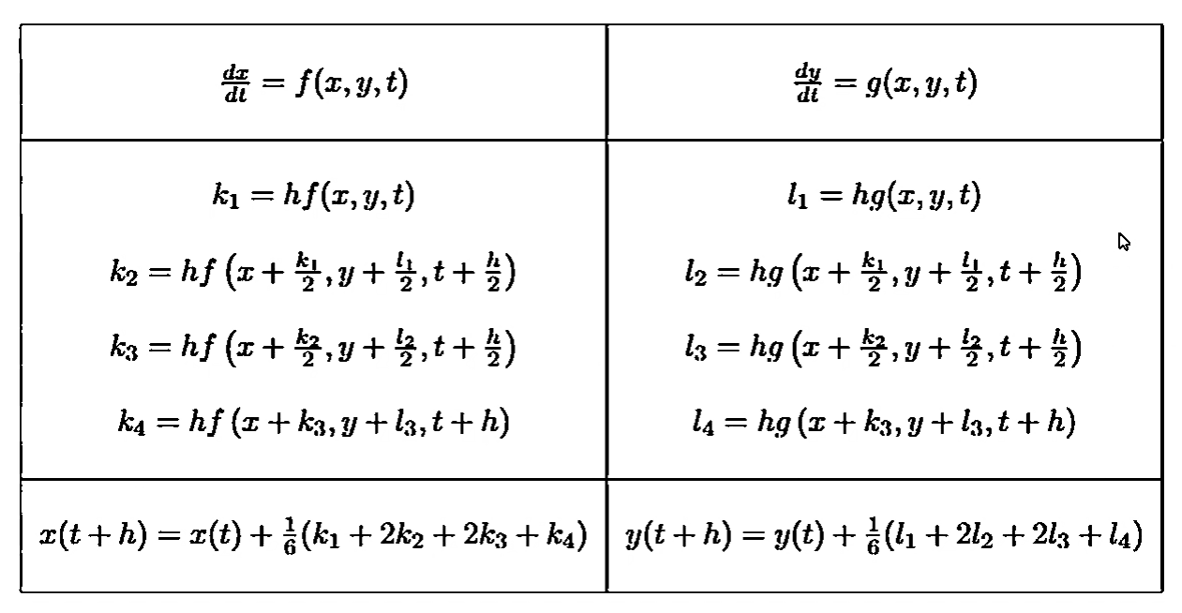
\includegraphics[width=\linewidth]{Tab1.png}
				Tabla 1. PROCEDIMIENTO PARA RESOLVER UN SISTEMA DE 2 E.D. DE PRIMER ORDEN
				\centering
			\end{figure}
		\end{frame}

		\subsection{Ejercicio}
			\begin{frame}{Ejercicio:}
				Haz un programa que calcule la posición y de un objeto en caída libre:
				$$ \frac{dy^2}{dt} = -g $$
				Tomando la ecuación diferencial y definiendo $ v_y = \frac{dy}{dt} $, la convertimos en el siguiente
				sistema de ecuaciones diferenciales
				$$ \frac{dy}{dt} = v_y \qquad \frac{dv_y}{dt} = -g $$
			\end{frame}
			
			\begin{frame}
				Utiliza el método de Runge-Kutta y considere que:
				\begin{itemize}
					\item $ g = 9.81 m/s^2 $
					\item $ y_0 = 100 m $
					\item $ v_0 = 0 m/s $
					\item $ t_0 = 0 s $
					\item $ t_f = 10 s $
				\end{itemize}
			\end{frame}

			\subsubsection{Solucion exacta:}
				\begin{frame}{Solucion exacta:}
					$$ v = -gt $$
					$$ y = \frac{-gt^2}{2} + 100 $$

				\end{frame}
				
%──────────────────────────────────────────────────────────────────────────────────────────────────────────────────────────────────────────

	\section{SPLINES}
		\begin{frame}{SPLINES}
			Los Splines son un método de interpolación que minimiza la curvatura general de
			la superficie a aproximar, resultando en una superficie suave que pasa exactamente
			por los puntos deseados.
			Una función Spline está formada por varios polinomios, cada uno definido sobre
			un subintervalo, que se unen entre sí obedeciendo a ciertas condiciones de continuidad.
		\end{frame}

		\begin{frame}
			para poder realizar esta interpolación necesitaremos valores asociados, $y_i$, 
			a unos puntos base, $X_i$:
			\begin{table}[h!]
				\centering
				\begin{tabular}{c|    c    c    c}
					$ x_i $ & $x_0$ & \dots & $x_{n-1}$ \\\hline
					$ y_i $ & $y_0$ & \dots & $y_{n-1}$ \\						
				\end{tabular}
			\end{table}
			El grado de un Spline viene determinado por el grado más alto de todos los polinomios 
			que forman el Spline, en sus intervalos de definición.
			$$ S(x) = 
			\left\lbrace\begin{array}{cccc}
				S_0(x) &  & [x_0,x_1] \\
				S_1(x) &  & [x_1,x_2] \\
				 \vdots &  & \vdots \\
				S_{n-1}(x) &  & [x_{n-2},x_{n-1}]
		    \end{array}\right.
			$$
		\end{frame}

		\begin{frame}{SPLINES CUBICOS}
			Un Spline cubico estan compuestos por polinomios de grado menor o igual a 3.
			Los polinomios por los que está formada $ S(x) $ tienen la forma:
			$$ S_i(x) = a_ix^3 + b_ix^2 + c_ix + d_i, $$
			Por lo que vemos que en cada polinomio $ S(x) $ tenemos 4 variables desconocidas $a_i$, $b_i$, $c_i$ y $d_i$, por lo que, teniendo $n$ puntos, encontramos:
			$$ (n-1)*4 $$ 
			variables que son necesarias para encontrar los $ n-1 $ polinomios.
		\end{frame}

		\begin{frame}
			Estas variables se pueden encontrar creando un sistema de ecuaciones con las siguientes condiciones:
			\begin{itemize}
				\item Condiciones de interpolación \\
					 $ S_i(x_i) = y_i $, i = 0, 1, 2, …, $n-1$
				\item Condiciones de suavidad (en nodos interiores)\\
					 $ S'_i(x_{i+1}) = S'_{i+1}(x_{i+1}) $, i = 1, 2, …, $n-2$
					 $ S''_i(x_{i+1}) = S''_{i+1}(x_{i+1}) $, i = 1, 2, …, $n-2$ 
				\item Splines naturales\\
					 $ S''_0(x_0) = 0 $ y $ S''_{n-1}(x_{n-1}) = 0 $
			\end{itemize}
		\end{frame}

		\begin{frame}
			Si consideramos que tenemos 4 puntos entonces las ecuaciones que para obtener las variables serian:\\
			\begin{table}[h!]
				\centering
				\begin{tabular}{c    c	 c}
					$ S_0(x_0) = y_0 \quad (1) $ & $ S'_0(x_1) = S'_1(x_1) \quad (7) $ \\
					$ S_0(x_1) = y_1 \quad (2) $ & $ S'_1(x_2) = S'_2(x_2) \quad (8) $ \\
					$ S_1(x_1) = y_1 \quad (3) $ & $ S''_0(x_1) = S''_1(x_1) \quad (9) $ \\
					$ S_1(x_2) = y_2 \quad (4) $ & $ S''_1(x_2) = S''_2(x_2) \quad (10) $ \\	
					$ S_2(x_2) = y_2 \quad (5) $ & $ S''_0(x_0) = 0 \quad (11) $ \\
					$ S_2(x_3) = y_3 \quad (6) $ & $ S''_2(x_3) = 0 \quad (12) $ \\
				\end{tabular}
			\end{table}
		\end{frame}

		\begin{frame}
			Entonces del sistema de ecuaciones anterior obtendríamos los polinomio de tercer grado que unen los n puntos dados.
			$$ S(x) = 
			\left\lbrace\begin{array}{cccc}
				a_0x^3 + b_0x^2 + c_0x + d_0 = 0 &  & [x_0,x_1) \\
				a_1x^3 + b_1x^2 + c_1x + d_1 = 0 &  & [x_1,x_2) \\
				a_2x^3 + b_2x^2 + c_2x + d_2 = 0 &  & [x_{2},x_{3}]
		    \end{array}\right.
			$$
		\end{frame}

%──────────────────────────────────────────────────────────────────────────────────────────────────────────────────────────────────────────

	\section{SIMPSON}
		\begin{frame}{SIMPSON}
			El Método de Simpson es una aproximación numérica que busca encontrar la solución a una 
			integral definida.
			\vspace{0.5cm}
			El Método sustituye a la curva por una serie de arcos contiguos, cada uno de estos arcos es 
			un arco de parábola de eje vertical. Esto nos lleva a aproximar el área bajo la curva 
			mediante la suma de las áreas bajo cada arco de parábola.
		\end{frame}

		\begin{frame}
			Una forma de aproximar una integral definida en un intervalo $[a,b]$ es mediante la regla del 
			trapecio, es decir, que sobre cada subintervalo en el que se divide $[a,b]$ se aproxima $f$ 
			por un polinomio de primer grado, para luego calcular la integral como suma de las áreas de 
			los trapecios formados en esos subintervalos . El método utilizado para la regla de Simpson 
			sigue la misma idea, pero aproximando los subintervalos de $f$ mediante polinomios de segundo 
			grado.	
		\end{frame}

		\begin{frame}{SIMPSON 1/3}
			\begin{figure}[H]
				\centering
				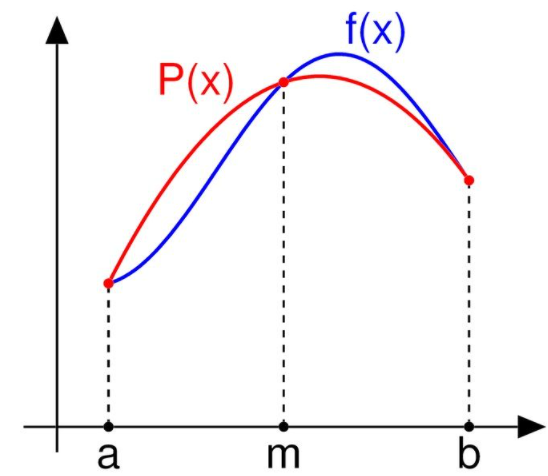
\includegraphics[scale=0.4]{11.png}
				\caption{REGLA DE SIMPSON 1/3}
				\centering
			\end{figure}
		\end{frame}

		\begin{frame}
			Esta sigue método sigue una aproximación para encontrar el resultado que es
			$$\int_{a}^{b} f(x)dx \approx \dfrac{b-a}{6}[f(a) + 4f(m) + f(b)]$$
			Donde se puede remplazar en la 8expresión $\dfrac{b-a}{2}$ como $h$ y se llega a la expresión 
			del método por la cual se calcula la aproximación de la integral definida.
			$$\int_{a}^{b} f(x)dx \approx \dfrac{h}{3}[f(a) + 4f(m) + f(b)]$$
			Donde $ m = a + h $
		\end{frame}

		\begin{frame}
			Pero esto también se puede aplicar par un numero n de particiones no solo para 2, la formula 
			teniendo es:
			$$ \int_{a}^{b} f(x)dx \approx \frac{b-a}{3n}\left(f(x_0) + 4\sum_{i=1,3,5}^{n-1}f(x_i) + 2\sum_{i=2,4,6}^{n-2}*f(x_i) + f(x_n)\right)$$
			Donde $ h = \frac{b-a}{n} $, $x_0 = a $ y $ x_n = b $, tendríamos la expresión para una aplicación múltiple:
			$$ \int_{a}^{b} f(x)dx \approx \frac{h}{3}\left(f(x_0) + 4\sum_{i=1,3,5}^{n-1}f(x_i) + 2\sum_{i=2,4,6}^{n-2}*f(x_i) + f(x_n)\right)$$
		\end{frame}

		\begin{frame}{REGLA DE SIMPSON 3/8}
			La regla de 3/8 de Simpson es similar a la regla de 1/3 de Simpson, con la única diferencia 
			de que, para la regla de 3/8, el interpolante es un polinomio cúbico. Aunque la regla de 3/8 
			utiliza un valor de función más y es aproximadamente dos veces más precisa que la regla de 
			1/3, y consiste en subdividir el intervalo $[a,b]$ en 3 subintervalos
			\begin{figure}[H]
				\centering
				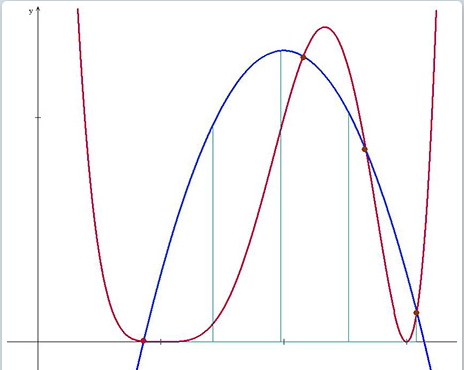
\includegraphics[scale=0.32]{12.png}
				\caption{REGLA DE SIMPSON 3/8}
				\centering
			\end{figure}

		\end{frame}
		
		\begin{frame}
			La fórmula de aproximar del método es de 
			$$\int_{a}^{b} f(x)dx \approx \dfrac{3h}{8}[f(a) + 3f(x_m) + 3f(x_n) + f(b)]$$
			Donde $h = \dfrac{b-a}{3}$ y donde $x_m = a+h $ y $x_n = x_m+h$. 
		\end{frame}
		
	\section{Referencias}
		\begin{frame}{Referencias}
			\centering
			\begin{thebibliography}{10}
				\bibitem{bib:item1} Métodos Numéricos para la enseñanza, Método de Simpson\\ 
								Recuperado 13 de Diciembre de 2021, de \\
								\href{https://multimedia.uned.ac.cr/pem/metodos_numericos_ensenanza/glosario/mod4.html}{Pagina web}
				\bibitem{bib:item2} Juan Carrillo (5 de Marzo del 2020), Método de Simpson\\ 
								Recuperado 13 de Diciembre de 2021, de \\
								\href{https://www.freecodecamp.org/espanol/news/la-regla-de-simpson-la-formula-y-como-funciona/}{Pagina web}
				\bibitem{bib:item3} Método de Runge Kutta\\
								Recuperado 13 de Diciembre de 2021, de \\
								\href{https://esimecuanalisisnumerico.wordpress.com/2014/05/06/metodo-numerico-de-runge-kutta/}{Pagina web}
				\bibitem{bib:item4}	Procedimientos numéricos, Ecuación diferencial de sgundo orden, Runge Kutta\\
								Recuperado 13 de Diciembre de 2021, de \\
								\href{http://www.sc.ehu.es/sbweb/fisica_/numerico/diferencial/segundo.html}{Pagina web}
			\end{thebibliography}
		\end{frame}

		\begin{frame}
			\centering
			\begin{thebibliography}{10}
				\bibitem{bib:item5}	Interpolación con funciones splines, Método de Splines\\
								Recuperado 13 de Diciembre de 2021, de \\
								\href{http://www4.ujaen.es/~angelcid/Archivos/An_Met_Num_INFORMATICA/Splines.pdf}{Pagina web}
				\bibitem{bib:item6} INTERPOLACION SPLINE Y APLICACIÓN A LAS CURVAS DE NIVEL, Método de Splines\\ 
								Recuperado 13 de Diciembre de 2021, de \\
								\href{http://diposit.ub.edu/dspace/bitstream/2445/122512/2/memoria.pdf}{Pagina web}
			\end{thebibliography}
		\end{frame}

\end{document}